%%%%%%%%%%%%%%%%%%%%%%% file template.tex %%%%%%%%%%%%%%%%%%%%%%%%%
%
% This is a general template file for the LaTeX package SVJour3
% for Springer journals.          Springer Heidelberg 2010/09/16
%
% Copy it to a new file with a new name and use it as the basis
% for your article. Delete % signs as needed.
%
% This template includes a few options for different layouts and
% content for various journals. Please consult a previous issue of
% your journal as needed.
%
%%%%%%%%%%%%%%%%%%%%%%%%%%%%%%%%%%%%%%%%%%%%%%%%%%%%%%%%%%%%%%%%%%%
%
% First comes an example EPS file -- just ignore it and
% proceed on the \documentclass line
% your LaTeX will extract the file if required
\begin{filecontents*}{example.eps}
%!PS-Adobe-3.0 EPSF-3.0
%%BoundingBox: 19 19 221 221
%%CreationDate: Mon Sep 29 1997
%%Creator: programmed by hand (JK)
%%EndComments
gsave
newpath
  20 20 moveto
  20 220 lineto
  220 220 lineto
  220 20 lineto
closepath
2 setlinewidth
gsave
  .4 setgray fill
grestore
stroke
grestore
\end{filecontents*}
%
\RequirePackage{fix-cm}
%
%\documentclass{svjour3}                     % onecolumn (standard format)
%\documentclass[smallcondensed]{svjour3}     % onecolumn (ditto)
\documentclass[smallextended]{svjour3}       % onecolumn (second format)
%\documentclass[twocolumn]{svjour3}          % twocolumn
%
\smartqed  % flush right qed marks, e.g. at end of proof
%
\usepackage{amsmath,amssymb,amsfonts}
\usepackage{graphicx}
\usepackage[justification=centering]{caption}
%
% \usepackage{mathptmx}      % use Times fonts if available on your TeX system
%
% insert here the call for the packages your document requires
%\usepackage{latexsym}
% etc.
%
% please place your own definitions here and don't use \def but
% \newcommand{}{}
%
% Insert the name of "your journal" with
% \journalname{myjournal}
%
\begin{document}

\title{Performance Evaluation of URLLC in 5G based on Stochastic Network Calculus\thanks{Supported by program National Natural Science Foundation of China (Nos.61872044,61502040). Beijing Municipal Program for Excellent Teacher Promotion (No.PXM2017\_014224.000028). Beijing Municipal Program for Top Talent Cultivation (CIT\&TCD201804055). Qinxin Talent Program of Beijing Information Science and Technology University.}}

%\subtitle{Do you have a subtitle?\\ If so, write it here}

%\titlerunning{Short form of title}        % if too long for running head

\author{Shengcheng Ma         \and
        Xin Chen              \and
        Zhuo Li               \and
        Ying Chen              %etc.
}

%\authorrunning{Short form of author list} % if too long for running head

\institute{F. Shengcheng Ma\at
              Beijing Information Science and Technology University, Beijing, China\\
              Tel.: +86-18510412330\\
              %Fax: +123-45-678910\\
              \email{mashengcheng@163.com}           %  \\
%             \emph{Present address:} of F. Author  %  if needed
           \and
           S. Xin Chen \at
              Beijing Information Science and Technology University, Beijing, China
           \and
           T. Zhuo Li \at
              Beijing Information Science and Technology University, Beijing, China
              \email{lizhuo@bistu.edu.cn}
           \and
           F. Ying Chen \at
              Beijing Information Science and Technology University, Beijing, China
}

\date{Received: date / Accepted: date}
% The correct dates will be entered by the editor


\maketitle

\begin{abstract}
Ultra-reliable low latency communications (URLLC) is one of the most important scenarios in 5G.
URLLC with strict latency and reliability requirements is widely used in delay-sensitive application such as self-driving.
As the 3GPP claims, the URLLC is amenable to 99.999\% transmission correctness and within 1ms delay bound.
How to meet the requirements of reliability and latency is still an open issue.
Few efforts have been made to applying a theoretical method to analyze the delay bound.
Stochastic network calculus is an elegant way to obtain the delay bound based on traffic models and service guarantees.
In this paper, we take the character of 5G architecture into account and use the stochastic network calculus to analyze the delay in URLLC.
A tandem model describing the communication in the 5G network is built, and parameters which have an influence on the delay are analyzed.
Numerical results are presented to verify the correctness of the delay analysis.
We investigate how to optimize the parameters to reduce the delay, which would provide valuable guidelines for the design of URLLC architecture.
\keywords{5G \and URLLC \and Stochastic Network Calculus \and Delay Analysis}
% \PACS{PACS code1 \and PACS code2 \and more}
% \subclass{MSC code1 \and MSC code2 \and more}
\end{abstract}

\section{Introduction}
\label{intro}
5G communication technology appeared for the first time with the 2018 Pyeongchang Winter Olympics in South Korea.
It helped audiences watch the live broadcast continuously and smoothly.
According to the 5G standard schedule announced by the International Telecommunication Union (ITU), 5G will begin commercialization in 2020
\cite{standard1}.
5G wireless networks are designed to support diverse and complicated scenarios.
The third generation partnership project (3GPP) classifies these different scenarios into three big categories: enhanced mobile broadband (eMBB), massive machine type communications (mMTC), and ultra-reliable low-latency communications (URLLC) \cite{standard2}.

Among them, URLLC is widely used in self-driving, mission-critical application, and some delay sensitive systems.
It has stringent requirements for the delay and reliability in the 5G New Radio (NR) systems.
The key requirements of URLLC as claimed by the 3GPP are to ensure the latency of user plane data less than 1ms, meanwhile to keep reliability not less than 99.999 percent \cite{article1}. %It is about 99.999 percent packet reception .
Such stringent delay requirement needs new 5G NR technology to bridge the gap.
Although existing 4G LTE (Long Term Evaluation) networks can achieve reliability goals, the cost is some dozens of milliseconds of delay.
That is far from the criteria of URLLC, so the delay becomes the bottleneck and this problem needs to be solved.
Many academies and companies have proposed some engineering solutions to minimize the delay, such as the HARQ retransmission or grant-free technology.
However, how to analyze the generation of delay from a theoretical perspective and propose a strategy to effectively reduce the delay is an important research subject.

Stochastic network calculus (SNC) theory is an effective tool for delay performance analysis.
SNC is a continuous development method to analyze network traffic characteristic and evaluate performance\cite{book1}.
Different from queuing theory, SNC permits some packets to violate the desired performance.
This feature can better take advantage of statistical multiplexing gains\cite{article2}.
To deal with random service and statistical guarantee, SNC theory comes into being with a large number of stochastic processes and network traffic models.
SNC theory can process service guarantee analysis of communication networks, such as delay and backlog.
Therefore, we utilize the SNC method to analyze the delay of the 5G URLLC transmission in this paper.

We use stochastic arrival curve to describe the process that user equipment (UE) data sends to gNodeB (gNB) side.
It represents the communication in Radio Access Network (RAN).
According to the 5G network topology architecture, we can deduce the rest stages of data transmission from gNB to cloud server.
Every stage of stochastic arrival curve characterizes the delay property, so the whole delay of URLLC system is comprised by delays generated from UE to the cloud server.

Since the standard of URLLC has not yet been formulated, various technologies are in the testing stage.
The existing performance evaluation research is only for a specific implementation.
In order to propose a compatible analysis method, we make an attempt to attack this challenge.
Our main contributions of this paper can be summarized as follows:

1) We build a tandem model to simulate 5G network architecture.
In this model, we can analyze the data transmission from UE to cloud server.
We use stochastic service process and concatenation property to analyze the latency.

2) To meet the needs of low latency and high availability for analyzing URLLC, we propose corresponding analysis methods.
We obtain a latency bound of gNB which is suit for analyzing delay in RAN.
Furthermore, we deduce a latency bound of URLLC to analyze the whole network latency.
To analyze the reliability of the network, we provide a stochastic error process which can express the block error rate.
We also investigate the impacts of block error rate on latency and propose a delay boundary analysis method.
%For delay analysis, stochastic latency bound for URLLC network is obtained.

3) Based on our analysis, we can find out what parameters are the key factors affecting the delay.
Delay analysis and strategy for reducing latency have valuable theoretical guidance for the design of URLLC deployment.
In order to meet stringent delay requirements, it provides guidelines for how to allocate resources.

The rest of this paper is organized as follows.
Section II summarizes related work of URLLC technology and stochastic network calculus.
We present a tandem network model to describe URLLC in Section III.
In particular, we illustrate the architecture of this system and analyze the causes of the delay in this section.
In section IV, we introduce the experimental environment and analyze the relationship between latency and main factors.
We conclude this paper in Section V.

\section{Related Work}
\label{sec:1}
Because the standard of URLLC has not been worked out, many researchers have put forward different solutions for the design of URLLC.

Research focuses on how to design and implement URLLC to meet the performance requirements.
A design without intervention in the baseband/PHY layer for URLLC is to use interface diversity and integrate multiple communication interfaces.
Jimmy and his colleagues proposed an analytical framework that combines traditional reliability models with technology-specific latency probability distributions\cite{article_interface}.
In this way, they were able to estimate the performance in terms of latency and reliability in such an integrated communication system.
To guarantee a low end-to-end delay with low jitter over combined internet and wireless interfaces,
the article \cite{article_multiconnectivity} presents a new round trip time (RTT) skew control controller with multiple-input multiple-output(MIMO).
This controller's advantage is that it solves the data flow split problem at the controlling node.
Jaya Rao and Sophie Vrzic proposed an approach to adopt packet duplication (PD) method to satisfy the latency and reliability requirements\cite{article_PD}.
PD technology generates multiple instances and sends them simultaneously in multiple unrelated channels.
The receiver selects the best packet according to the channel condition in order to achieve better transmission reliability.
This PD technique can provide a cost-effective solution without increasing the complexity in the RAN.

In terms of resource allocation and energy efficiency, there are also some research on URLLC.
How the frequency resource will be allocated to the user to send data in URLLC scenario.
That is an interesting study which is plunged by Anand A and De Veciana G\cite{article_Anand}.
Based on the 5G standard technology Orthogonal Frequency Division Multiple Access (OFDMA), they built a One Shot Transmission model.
Adopting queuing theory analysis, they found out that a small bandwidth over a longer duration is better than a large swath of bandwidth for short duration in One Shot Transmission system.
Green energy saving is getting more and more attention.
The article \cite{article_Energy} provides a coordinated on-off switching scheme across a set of adjacent gNBs.
The gNBs share a sleep schedule among themselves.
If the gNBs have lower traffic and fewer connected UEs, they will be set to the OFF mode.
This On-Off mode is more energy-efficient than traditional mode on the premise of guaranteeing the time delay.

Because URLLC has strict requirements for delay and reliability, it is very meaningful to evaluate the performance of URLLC.
Joachim et al. provide an achievable latency bound evaluation in their article\cite{article_joachim}.
They compare the latencies for different configurations in 5G RAN transmission.
The configuration contains FDD, TDD, frequency numerologies and usage of slots.
According to the analysis, a frequency with higher numerology can be used to reduce the latency.
An article derived from HUAWEI company proposes a grant-free mode uplink transmission mechanism\cite{proc_Huawei}.
Grant-free transmission grants dynamically without scheduling request.
This mode is poised to meet the reliability requirement of URLLC in uplink transmission.
By simulating random arriving from different numbers of active UEs, the reliability can be improved after adopting the grant-free mode with increasing retransmission.

In order to satisfy the key requirements including latency and reliability, some state-of-the-art solutions have been discussed in \cite{article_Achieving}\cite{article_Wireless}\cite{article_Introduction}\cite{article_Physical}.
These technologies contain fast HARQ retransmission, MIMO, beam forming, diversity interfaces, D2D communication, Ultra Density Network and so on.
Some of these technologies can be employed alone to promote performance, and others need to be combined together to achieve better results.
They all mentioned the design of frame structures.
That was because low latency and high reliability are contradictory.
This requires more flexible frequency and time division.

Stochastic network calculus is a very practical tool, and it has a good practical effect in performance analysis and theoretical boundary calculation.
Li and Jiang \cite{article_jiang_power} analyzed the throughput performance on the wireless-powered communication system.
They considered the delay as a constrained condition.
The stochastic traffic arrival was adopted to derive the cumulative data transmission capacity.
M. Fidler and his coauthors \cite{proc_MF_Estimation} used stochastic service process to analyze the end-to-end delay performance of TCP.
The estimation method of closed-loop flow was implemented by random service process in this paper.
They considered both backlog and delay by using stochastic network calculus.
In reference \cite{article_beiyou_lei1}, the performance of wireless finite-state Markov channel was analyzed.
The delay boundary was derived based on the moment generating functions (MGF).
Xin Chen's team focused on LTE network and researched the resource allocation to guarantee the delay performance \cite{article_si_yuan}.
The delay was constrained by the difference value between stochastic arrival curve and stochastic service curve.
Reference \cite{article_MF_jiang} is a collaboration between Fidler M and Jiang.
It mainly applies SNC theory to analyze the delay boundary of multi-server systems.

\section{System Model}

To build a system model, we need to consider two points. The first is how to reflect the real situation of 5G networks in our system. The article \cite{article_Energy} and \cite{article_joachim} are both use the concatenate model to describe the composition of the delay in URLLC networks. The second point is that does the SNC theory suit for the performance analysis in URLLC communication? Guang Yang, Ming Xiao, and H. Vincent Poor have done similar work by using SNC theory in Low-Latency Millimeter-Wave Communication\cite{article_Millimeter}. Although the Millimeter-Wave is not the only way to implement URLLC, it still can prove the SNC theory can accomplish the delay analysis. To sum up these two points, we make an attempt to combine SNC and the tandem model to analyze the performance in 5G URLLC. Furthermore, system reliability will be discussed in this section.

\subsection{URLLC Network Architecture}
\label{sec:2}
Generally speaking, 5G network includes Standalone networking (SA) and Non-standalone networking (NSA).
The SA mode is the establishment of whole new 5G network, while the NSA mode is the combination of 5G and 4G LTE.
According to the implementation technology of the core network, the NSA mode can further be divided.
In order to simplify the system model, we only discuss the case of 5G standalone network.

We consider URLLC network as a concatenate system from UE to Cloud.
The 4G LTE network is composed by UE, RRU (Radio Remote Unit), BBU (Building Baseband Unit), the EPC (Evolved Packet Core) which is the LTE's core network, and the endpoint is cloud servers.
Different from 4G LTE, 5G networks are composed by UE, gNB, NGC and Cloud.
The gNB contains three parts, which are AAU (Active Antenna Unit), DU (Distributed Unit), and CU (Centralized Unit).
AAU takes the place of the original RRU and combines some physical layer processing functions of BBU.
The BBU function of 4G will be rebuilt into DU and CU in 5G.
CU provides the service convergence function in the access side. It focuses on the low real-time capabilities of the protocol stack and adopts a centralized deployment.
DU mainly provides data access function to the terminal, including radio frequency and partial signal processing. DU concentrate on the high real-time capabilities of the transport requirements and suit for a distributed deployment method.
The NGC (Next Generation Core Network) as Core Network in 5G replace the EPC. 5G NGC is based on SDN/NFV technology and designed to better fit the cloud platform.
The architecture is depicted as Fig.\ref{fig_architecture}.
\begin{figure*}[htbp]
\centering
  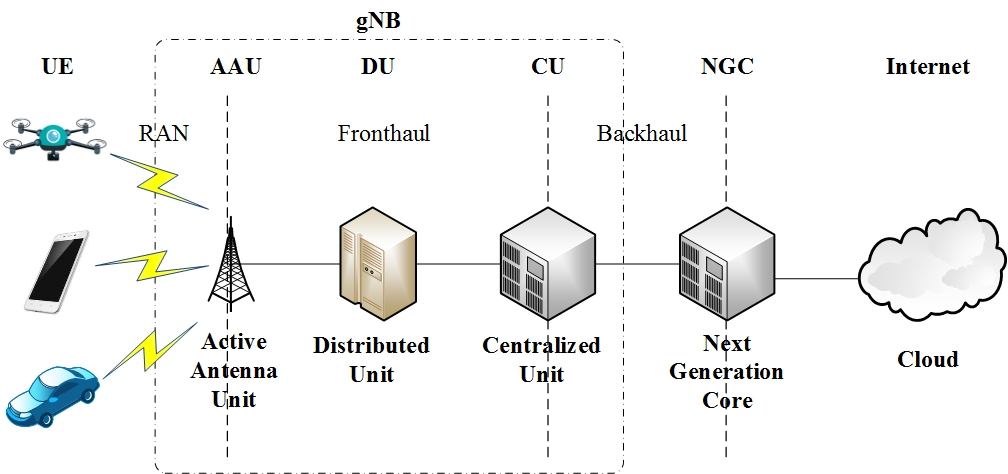
\includegraphics[width=0.75\textwidth]{5G_delay_en.jpg}
\caption{5G network architecture.}
\label{fig_architecture}
\end{figure*}


\subsection{Delay of URLLC Network}

In this part, we discuss the latency mainly on the User Plane (UP) rather than the Control Plane (C-Plane).
That is because the delay requirement of user plane is higher than that of control plane.
UP latency is the communication time between UE and network nodes when transmission and reception of the data at the corresponding IP layer, whereas the C-Plane latency is the time spend on radio resource allocating and state switching from idle to active.
%Compared with UP latency, the C-Plane delay is tiny.
The results of comparison between UP latency and C-Plane have been discussed in reference \cite{article_Energy}.
To simplify the analysis, we mainly consider the delay generated by the User Plane.

UE devices firstly access to AAU. The AAU is actually a part of the base station. This part of the communication belongs to RAN.
UE's data will be accepted by AAU, and AAU put forward the data to DU.
There are two situations when data arrive at DU.
If CU and DU are deployed together, the data can arrive at CU immediately. Otherwise, the data will be sent to CU from DU.
The communication from AAU to CU belongs to fronthaul.
The data leave CU and continue upward to the NGC. This part of the communication is called backhaul.
NGC will process the data and it will take some time.
Finally, NGC sends the data to Cloud servers. The unidirectional transmission is finished.

Consequently, the whole delay or latency in 5G system is contributed by the time processing of RAN, fronthual, backhaul, Core Network, and Cloud server. It can be expressed as (\ref{eq_urllc_delay_composition}).
\begin{equation}\label{eq_urllc_delay_composition}
T_{Total} = T_{RAN} + T_{Fronthaul} + T_{Backhaul} + T_{NGC} + T_{Cloud}
\end{equation}
where
\begin{itemize}
\item $T_{RAN}$ is the time cost by physical layer transmission between UEs and AAU.
\item $T_{Fronthaul}$ is the delay between AAU to CU. It is the time taken in gNB.
\item $T_{Backhaul}$ is the time taken to communication between gNB to NGC.
\item $T_{NGC}$ is the delay taken place in NGC.
\item $T_{Cloud}$ is the latency which data transmission between NGC and Cloud server.
\end{itemize}
To meet the URLLC key requirement, it is essential to study $T_{Total}$.
%we should do a good job of studying $T_{Total}$.

\subsection{Problem Description}
The data is transferred from UE, through each node, and finally to the cloud.
According to the requirement of URLLC, the random latency \cite{article_MF_Random} can be described as (\ref{eq_urllc_delay_problem}):
\begin{equation}\label{eq_urllc_delay_problem}
P\{delay > d \} < \epsilon
\end{equation}
The delay should be within 1ms, so the value of $d$ should be less than 1 and the unit is millisecond (ms).
The $\epsilon$ is defined as a very small probability.
Equation(\ref{eq_urllc_delay_problem}) represents a 5G URLLC network that successfully transfers data and meets the delay requirements.

\subsection{Basics of Stochastic Network Calculus}
In SNC theory, the min-plus algebra is applied to analyze queuing system.
Let $\mathcal{F}$ denotes the set of non-negative non-decreasing functions and $\mathcal{\bar{F}}$ denotes the set of non-negative non-increasing function.
We employ the cumulative process to represent amount of traffic flow.
Arrival process, departure process and service process are denoted as $A(t)$, $D(t)$, and $S(t)$ respectively.
For any $0 \leq s \leq t, A(0)=0, A(s,t) = A(t) - A(s)$, and practical significance of $A(t)$ is the cumulative arrival data at time $t$.
It is the same for $D(t)$ and $S(t)$.
Some fundamental definitions of curve are well described in the literature \cite{book1}.
We utilize and expand the following in this paper.

\begin{definition}\label{def_SAC}
{\bfseries (Stochastic Arrival Curve)}.
A flow is said to have a stochastic arrival curve $\alpha\in\mathcal{F}$ with bounding function $f\in\mathcal{\bar{F}}$, denoted by $A(t) \sim <f,\alpha>$, if for all $t \geq 0$ and all $x\geq0$ there holds
\begin{equation}\label{eq_sac}
P\Bigl\{\sup_{0\leq s \leq t}\{A(s,t) - \alpha(t-s)\} > x \Bigr\} \leq f(x).
\end{equation}
\end{definition}
Where $\alpha(\tau)$ is the stochastic arrival curve, and it denotes the maximum of flow $A(\tau)$.
Function $f(x)$ denotes the violation probability.
It assumes that the stochastic arrival curve $\alpha(\tau)$ may be exceeded by arrival process $A(\tau)$ in sometimes, but the probability of being exceeded is constrained by the boundary function $f(x)$.

\begin{definition}\label{def_SSC}
{\bfseries(Stochastic Service Curve)}. A system $S$ is said to provide a stochastic service curve $\beta\in\mathcal{F}$ with bounding function $g \in \mathcal{\bar{F}}$, denoted by $S \sim<g, \beta>$, if for all $t\geq0$ there holds
\begin{equation}\label{eq_ssc}
P\Bigl\{\sup_{0\leq s \leq t}[A\otimes\beta(s) - D(s)] > x \Bigr\} \leq g(x).
\end{equation}
\end{definition}

The symbol $\otimes$ represents the cumulative min-plus convolution operation.
Where
\begin{equation}\label{eq_convolution}
A\otimes\beta(t) = \inf_{0 \leq s \leq t}\{A(s)+\beta(s,t)\}
\end{equation}
$\beta(t)$ is the stochastic service curve which means the worst service capability provided by the server.
Similar to the stochastic arrival curve, the data that have been processed are probably more than the data departed.
The probability of producing exceeding data can be constrained by the boundary function $g(x)$.

Similarly as in (\ref{eq_ssc}), the departure process relates to the arrival and service process and it is described as
\begin{equation}\label{eq_departure}
D(t) \geq \inf_{0\leq s \leq t}\{A(s)+ S(s,t)\} =  A \otimes S(t).
\end{equation}
Where for all $s,t \geq 0$ and $s \leq t$.
That is also the concept of a dynamic server which mentioned in \cite{article1}.
From the (\ref{eq_departure}), we can better understand the relationship among arrival process, departure process and service process.
With these basic processes and curves, we can discuss the definition of the delay boundary.

\begin{definition}\label{def_delay_process}
{\bfseries(Latency Process)}.
Let $A(t)$ and $D(t)$ respectively be the arrival process and departure process.
The latency process $L(t)$ at time $t \geq 0$ is defined as
\begin{equation}\label{eq_delay_define}
L(t) = \inf\{d \geq 0 : A(t) \leq D(t+d)\}.
\end{equation}
\end{definition}

Equation (\ref{eq_delay_define}) express that latency $L(t)$ is the least value of $d$, and $d$ must meet the condition that the amount of arrival data at time $t$ is less than or equal to the departure data at time $t+d$.
It also means that the data do not leave the server immediately.
The duration of the data in server is the delay time.
In (\ref{eq_delay_define}), the arrival process $A(t)$ is less than or equal to the departure process $D(t+d)$.
It means that the data arrived in server at time $t$ are all leaving from server at time $t+d$.
If $A(t)$ is large than or equal to the departure process $D(t+d)$, that represents the data arrived at $t$ moment have not been completed by service during $d$ period of time.
Therefore, the $A(t)$ less than or equal to $D(t+d)$ situation is utilized to describe the shortest time that server takes for the data to be serviced.
That is the latency or delay.

According to the latency process definition, and utilizing stochastic arrival process and stochastic service process, so the stochastic latency bound has been defined at following.

\begin{lemma}\label{thrm_latency}{\bfseries (Stochastic Latency Bound)}
A system with an input process $A(t)$.
$A(t)$ is a stochastic arrival process with stochastic arrival curve $\alpha \in \mathcal{F}$ and bounded by function $f \in \mathcal{\bar{F}}$ (i.e., $A \sim <f, \alpha>$).
The system provides to the input a stochastic service process $S(t)$.
$S(t)$ is with stochastic service curve $\beta \in \mathcal{F}$ with bounding function $g \in \mathcal{\bar{F}}$ (i.e., $S \sim <g, \beta>$).
Then, for all $t\geq 0$ and $x \geq 0$, the Latency $L(t)$ is bounded by
\begin{equation}
P\{L(t)>h(\alpha+x, \beta)\}\leq f \otimes g(x)
\end{equation}
\end{lemma}
Where function $h(\alpha+x, \beta)$ denotes the maximum horizontal distance between $\alpha+x$ and $\beta$, the express $f \otimes g(x)$ represents the cumulative min-plus convolution operation of function $f$ and $g$.

\begin{lemma}\label{thrm_concatenation}{\bfseries (Concatenation Property)}
Considering a flow passes through a network of $N$ server nodes in tandem.
If each server nodes $n(=1,2,...,N)$ provides a stochastic service curve $S^{n}\sim<g^{n}, \beta^{n}>$ to its input, then the network guarantees to the flow a stochastic service curve $S\sim<g,\beta>$ with
\begin{equation}
\begin{split}
\beta(t)=\beta^{1}\otimes\beta^{2}\otimes\cdot\cdot\cdot\otimes\beta^{N}(t) \\
g(x)=g^{1}\otimes g^{2}\otimes\cdot\cdot\cdot\otimes g^{N}(t)
\end{split}
\end{equation}
\end{lemma}

\subsection{Model Building}
The network character of URLLC can be described as a dynamic server by stochastic processes as introducing in above.
The data sent by UE can be represented by the arrival process $A(t)$.
The service capacity provided by the network server node can be depicted as the stochastic service process $S(t)$.
As the assumption in equation (\ref{eq_urllc_delay_composition}), we consider the URLLC network is a tandem system.
Therefore, the delay of URLLC should fall in the concatenation characterization in SNC.

We consider that a UE's network flow passing through the gNB, CN and Cloud in tandem mode.
Each network node $k(=gNB, AAU, DU, CU, CN, Cloud)$ provides a stochastic service curve $S_{k}\sim<g_k, \beta_k>$ to its flow.
We first discuss about the gNB subsystem.
The gNB includes AAU, DU and CU, so $S_{AAU}(s,t)$, $S_{DU}(s,t)$ and $S_{CU}(s,t)$ are in series.
We use the same indices to denote the arrival and departure process of the respective systems.
Especially the source of data is from UE, so $A_{AAU}(t)$ as arrival process denotes the input data of AAU from UE in gNB subsystem.
The arrival process of DU $A_{DU}(t)$ actually equals to the departure process of AAU $D_{AAU}(t)$, where $A_{DU}(t) = D_{AAU}(t)$.
By the same token, $A_{CU}(t) = D_{DU}(t)$ similarly for CU server.
The departure process of CU is $D_{CU}(t)$.
It is also the departure process of the gNB subsystem.

\subsubsection{Delay of gNB}

Considering that the gNB subsystem is tandem deployed, we assume that the AAU server provides a $S_{AAU}(t)$ capacity to deal with the arrival data.
Applying (\ref{eq_departure}), the departure process can be represent as
\begin{equation} \label{eq_departure_AAU}
D_{AAU}(t)\geq A_{AAU}\otimes S_{AAU}(t).
\end{equation}
Similar to the departure process of AAU, we can get the process of DU
\begin{equation}\label{eq_departure_DU}
D_{DU}(t) \geq A_{DU}\otimes S_{DU}(t).
\end{equation}
Because of $A_{DU}(t) = D_{AAU}(t) = A_{AAU}\otimes S_{AAU}(t)$, we put (\ref{eq_departure_AAU}) into (\ref{eq_departure_DU}) to replace $A_{DU}(t)$ by $A_{AAU}\otimes S_{AAU}(t)$ and get
\begin{equation}\label{eq_departure_DU2}
D_{DU}(t) \geq (A_{AAU}\otimes S_{AAU}(t))\otimes S_{DU}(t).
\end{equation}
By recursive insertion, we can obtain
\begin{equation}\label{eq_departure_CU}
D_{CU}(t) \geq ((A_{AAU}\otimes S_{AAU}) \otimes S_{DU})\otimes S_{CU}(t).
\end{equation}
Applying the associativity of min-plus convolution, it holds that
\begin{equation}
\begin{split}
D_{CU}(t) &\geq ((A_{AAU}\otimes S_{AAU}) \otimes S_{DU})\otimes S_{CU}(t) \\
&\geq A_{AAU}\otimes (S_{AAU}\otimes S_{DU} \otimes S_{CU})(t).
\end{split}
\end{equation}
From the gNB subsystem perspective to see, $A_{AAU}(t)$ is the first input and $D_{CU}(t)$ is the last output of gNB.
Therefore, $A_{AAU}(t)$ equal to $A_{gNB}(t)$, and $D_{CU}(t)$ is the departure process of the gNB $D_{gNB}(t)$.
Then we can get gNB subsystem
\begin{equation}\label{eq_departure_gNB}
D_{gNB} \geq A_{AAU}\otimes (S_{AAU}\otimes S_{DU} \otimes S_{CU})(t).
\end{equation}
Assuming first-come first-served order, we use Definition.\ref{def_delay_process} and equation (\ref{eq_departure_gNB}), and let $L_{gNB}$ denotes the latency process of gNB, there holds
\begin{equation}\label{eq_latency_gNB}
\begin{split}
L_{gNB}(t) &= \inf\{d\geqslant0: A_{gNB}(t) - D_{gNB}(t+d) \leqslant 0 \} \\
 &= \inf\{d\geqslant0: A_{AAU}(t) - D_{CU}(t+d) \leqslant 0 \}  \\
 &= \inf\{d\geqslant0: A_{AAU}(t) \\
 &  - A_{AAU}\otimes (S_{AAU}\otimes S_{DU} \otimes S_{CU})(t+d) \leqslant 0 \}
\end{split}
\end{equation}

With Lemma.\ref{thrm_latency} and Lemma.\ref{thrm_concatenation}, the delay bound can be analysis by following theorem.
\begin{theorem}\label{crl_latency}{\bfseries (Latency Bound of gNB)}
In gNB subsystem, $A_{AAU}(t)$ is a stochastic arrival process with stochastic arrival curve $\alpha_{AAU}$, i.e. $A \sim <f_{AAU}, \alpha_{AAU}>$.
 $\alpha_{AAU} \in \mathcal{F}$, $f_{AAU} \in \mathcal{\bar{F}}$.
The server nodes in subsystem provide stochastic service process $S_{AAU}(t), S_{DU}(t), S_{CU}(t)$ respectively, i.e.
$S_{AAU} \sim <g_{AAU},\beta_{AAU}>, S_{DU}\sim <g_{DU},\beta_{DU}>, S_{CU}\sim <g_{CU}, \beta_{CU}>$.
And $\beta_{AAU},\beta_{DU},\beta_{CU} \in \mathcal{F}$, $g_{AAU}, g_{DU}, g_{CU} \in \mathcal{\bar{F}}$.
Then, for all $t\geq 0$ and $x \geq 0$, the Latency of gNB subsystem $L_{gNB}(t)$ is bounded by
\begin{equation}
\begin{split}
P\{L_{gNB}(t) \geq d\} &= P\{L_{gNB}(t) \geq h(\alpha_{AUU}+x, \beta_{gNB})\} \\
 &\leqslant f_{AAU}\otimes g_{gNB}(x)
\end{split}
\end{equation}
\end{theorem}
where service rate $\beta_{gNB}(t)=\beta_{AAU}\otimes \beta_{DU}\otimes \beta_{CU}(t)$, and bound function $g_{gNB}=g_{AAU}\otimes g_{DU}\otimes g_{CU}(x)$.


\begin{proof}:
Since the latency process Definition.(\ref{def_delay_process}) is defined as $L(t) = \inf\{d \geq 0 : A(t) \leq D(t+d)\}$,
event ${L(t)} > d$ implies event ${A(t)\leq D(t+d)}$.
We move $D(t+d)$ from right hand to left hand, and according to (\ref{eq_latency_gNB}), the latency bound of gNB can be hold as
\begin{equation}\label{eq_latencybound_gNB}
P\{L_{gNB}(t)>d\} \leqslant P\{A_{AAU}(t) - D_{CU}(t+d) \leq 0\}
\end{equation}

Then we focus on the $\{A_{AAU}(t) - D_{CU}(t+d)\}$ part. We put right hand of (\ref{eq_departure_gNB}) into this part, we can get
\begin{equation}\label{zm_1}
\begin{split}
 &A_{AAU}(t) - D_{CU}(t+d) \\
=&A_{AAU}(t) - A_{AAU}\otimes (S_{AAU}\otimes S_{DU}\otimes S_{CU})(t+d)\\
+&A_{AAU}\otimes (S_{AAU}\otimes S_{DU}\otimes S_{CU})(t+d)-D_{CU}(t+d)\\
\end{split}
\end{equation}

With the Lemma.\ref{thrm_concatenation}, utilizing the concatenation property we can obtain that
$S_{AAU}\sim<g_{AAU},\beta_{AAU}>$, $S_{DU}\sim<g_{DU},\beta_{DU}>$, $S_{CU}\sim<g_{CU},\beta_{CU}>$.
Stochastic service process convolution operation $(S_{AAU}\otimes S_{DU}\otimes S_{CU})$ means gNB subsystem provides maybe lower than $(\beta_{AAU}\otimes \beta_{DU} \otimes \beta_{CU})$ processing capacity,
but the violation probability in this case is limited by $g_{AAU}\otimes g_{DU}\otimes g_{DU}$.
Through applying (\ref{eq_ssc}), we denote $\beta_{gNB}$ equals to $(\beta_{AAU}\otimes \beta_{DU} \otimes \beta_{CU})$,
$g_{gNB}$ equals to $g_{AAU}\otimes g_{DU}\otimes g_{DU}$.
hence (\ref{zm_1}) can hold be
\begin{equation}\label{zm_2}
\begin{split}
 &A_{AAU}(t) - D_{CU}(t+d) \\
=&A_{AAU}(t) - A_{AAU}\otimes (\beta_{AAU}\otimes \beta_{DU}\otimes \beta_{CU})(t+d)\\
 &+A_{AAU}\otimes (\beta_{AAU}\otimes \beta_{DU}\otimes \beta_{CU})(t+d) - D_{CU}(t+d) \\
=&A_{AAU}(t) - A_{AAU}\otimes \beta_{gNB}(t+d) \\
 &+A_{AAU}\otimes \beta_{gNB}(t+d) - D_{CU}(t+d)
\end{split}
\end{equation}
According to (\ref{eq_convolution}), we replace $A_{AAU}\otimes \beta_{gNB}(t+d)$ by $\inf\{A_{AAU}(s)+\beta_{gNB}(t+d-s)\}$ in (\ref{zm_2}).
Consequently,
\begin{equation}\label{zm_3}
\begin{split}
 &A_{AAU}(t) - D_{CU}(t+d) \\
=&A_{AAU}(t) - A_{AAU}\otimes \beta_{gNB}(t+d) \\
 &+A_{AAU}\otimes \beta_{gNB}(t+d) - D_{CU}(t+d) \\
=&A_{AAU}(t) - \inf_{0\leqslant s \leqslant t+d}\{A_{AAU}(s)+ \beta_{gNB}(t+d-s)\} \\
 &+A_{AAU}\otimes \beta_{gNB}(t+d) - D_{CU}(t+d)\\
\leq&A_{AAU}(t) - A_{AAU}(s) - \beta_{gNB}(t+d-s)\} \\
 &+A_{AAU}\otimes \beta_{gNB}(t+d) - D_{CU}(t+d)  \\
\leq&A_{AAU}(s,t) - \alpha_{AAU}(t-s)\\
 &+\alpha_{AAU}(s,t)-\beta_{gNB}(t+d-s)\\
 &+A_{AAU}\otimes \beta_{gNB}(t+d) - D_{CU}(t+d)  \\
\end{split}
\end{equation}

We add $\alpha_{AAU}$ at step 4 in (\ref{zm_3}) to build stochastic arrival curve.
Based on the stochastic arrival curve (\ref{eq_sac}),$A_{AAU}(s,t) - \alpha_{AAU}(s,t)$ is less than or equal to $f_{AAU}$.
Applying stochastic service curve (\ref{eq_ssc}), $A_{AAU}\otimes \beta_{gNB}(t+d) - D_{CU}(t+d)$ is less than or equal to $g_{gNB}$.
With Theorum.\ref{thrm_latency}, we use $h(\alpha+x, \beta)$ replace the $d$. where $h(\alpha+x,\beta)$ is the maximum horizontal distance between $\alpha+x$ and $\beta$ for $x \geq 0$. The $h(\alpha,\beta)$ function implies the condition
\begin{equation}\label{condition}
\lim_{t\rightarrow\infty}[\alpha(t)-\beta(t)]\leq 0.
\end{equation}
we can obtain
\begin{align*}
&P\{L(t)>h(\alpha_{AAU}+x, \beta_{gNB})\} \\
&= P\{\{A_{AAU}(t) - D_{CU}(t+h(\alpha+x, \beta))\} > 0\}  \\
&\leqslant \sup_{0\leqslant s \leqslant t}\{A_{AAU}(s,t)-\alpha_{AAU}(t-s)\}  \\
&+\sup_{0\leqslant s \leqslant t+h(\alpha_{AAU}+x, \beta_{gNB})}\{A_{AAU}\otimes \beta_{gNB}(s)-D_{CU}(s)\} \\
&\leqslant f_{AAU}(t)+g_{gNB}(x) \\
&\leqslant \inf\{f_{AAU}(t)+g_{gNB}(x-t)\} \\
&\leqslant f_{AAU}\otimes g_{gNB}(x)
\end{align*}
Therefore, Theorem.\ref{crl_latency} is proved.
\end{proof}

\subsubsection{Delay of URLLC}

For mobile edge computing (MEC) deployment, CU can be the end of the transmission. That is because the computing resource and storage resource are located at CU.
The Theorem.\ref{crl_latency} is suitable for analyzing the delay of communication from UE to CU.
However, in order to comprehensively discuss the delay of URLLC system, we need to convert the destination from CU to Cloud.
By extending Theorem.\ref{crl_latency}, we can draw the whole URLLC system latency bound.
\begin{theorem}\label{crl_latency_urllc}{\bfseries (Latency Bound of URLLC)}
In 5G URLLC system, $A_{AAU}(t)$ is a stochastic arrival process with stochastic arrival curve $\alpha_{AAU}$, i.e. $A\sim<f_{AAU},\alpha_{gNB}>$. $\alpha_{AAU}\in\mathcal{F}$, $f_{AAU}\in\mathcal{\bar{F}}$.
The server nodes in URLLC system provide stochastic service process $S_{gNB}(t)$, $S_{NGC}(t)$ and $S_{Cloud}(t)$ respectively, i.e.
$S_{gNB}\sim<g_{gNB},\beta_{gNB}>$, $S_{NGC}\sim<g_{NGC},\beta_{NGC}>$, and $S_{Cloud}\sim<g_{Cloud},\beta_{Cloud}>$.
Service rate $\beta_{gNB},\beta_{NGC},\beta_{Cloud}\in\mathcal{F}$, $g_{gNB}, g_{NGC}, g_{Cloud}\in\mathcal{\bar{F}}$.
Then, for all $t\geq 0$ and $x \geq 0$, the Latency of URLLC system $L_{All}(t)$ is bounded by
\begin{equation}\label{eq_in_crl_2}
\begin{split}
P\{L_{All}(t) \geq d\} &= P\{L_{All}(t) \geq h(\alpha_{AUU}+x, \beta_{All})\} \\
 &\leqslant f_{AAU}\otimes g_{All}(x)
\end{split}
\end{equation}
\end{theorem}
where $\beta_{All}(t)=\beta_{gNB}\otimes \beta_{NGC}\otimes \beta_{Cloud}(t)$, and $g_{All}=g_{gNB}\otimes g_{NGC}\otimes g_{Cloud}(x)$.

\begin{proof}:
In the Theorem.\ref{crl_latency}, the gNB subsystem are constituted by AAU, DU and CU. In addition to gNB, the whole 5G URLLC system also include NGC and Cloud.
According to the concatenation property which mentioned in Lemma.\ref{thrm_concatenation}, then the network guarantees to the flow a stochastic service curve $S_{All}\sim<g_{All},\beta_{All}>$ with
\begin{equation}\label{eq_tandem_beta_top}
\beta_{All}(t)=\beta_{gNB}\otimes\beta_{CN}\otimes\beta_{Cloud}(t)
\end{equation}
where
\begin{equation}\label{eq_tandem_beta_gNB}
\beta_{gNB}(t)=\beta_{AAU}\otimes\beta_{DU}\otimes\beta_{CU}(t)
\end{equation}
actually
\begin{equation}\label{eq_tandem_beta_all}
\beta_{All}(t)=\beta_{AAU}\otimes\beta_{DU}\otimes\beta_{CU}\otimes\beta_{CN}\otimes\beta_{Cloud}(t)
\end{equation}
and
\begin{equation}\label{eq_tandem_g_top}
g_{All}(x)=g_{gNB}\otimes g_{CN}\otimes g_{Cloud}(x)
\end{equation}
where
\begin{equation}\label{eq_tandem_g_gNB}
g_{gNB}(x)=g_{AAU}\otimes g_{DU}\otimes g_{CU}(x)
\end{equation}
actually
\begin{equation}\label{eq_tandem_g_all}
g_{All}(x)=g_{AAU}\otimes g_{DU}\otimes g_{CU}\otimes g_{CN}\otimes g_{Cloud}(x)
\end{equation}
Based on latency process Definition.(3), the 5G URLLC system latency process can be defined as
\begin{equation}
L(t) = \inf\{d \geqslant 0: A_{AAU}(t) \leq D_{Cloud}(t+d)\}
\end{equation}
Latency bound of 5G URLLC is defined as
\begin{equation}
P\{L(t)\geq d\} = P\{A_{AAU}(t)-D_{Cloud}(t+d)\leq 0\}
\end{equation}
We also focus on $A_{AAU}(t)-D_{Cloud}(t+d)$ part.
where $D_{Cloud}\geqslant A_{AAU}\otimes S_{AAU}\otimes S_{DU}\otimes S_{CU}\otimes S_{NGC}\otimes S_{Cloud}$. Then we have
\begin{align*}
&A_{AAU}(t)-D_{Cloud}(t+d)\\
=&A_{AAU}(t)-A_{AAU}\otimes S_{AAU}\otimes S_{DU}\otimes S_{CU}\\
&\otimes S_{NGC}\otimes S_{Cloud}(t+d)\\
&+A_{AAU}\otimes S_{AAU}\otimes S_{DU}\otimes S_{CU}\\
&\otimes S_{NGC}\otimes S_{Cloud} -D_{Cloud}(t+d)\\
=&A_{AAU}(t)-A_{AAU}\otimes S_{gNB}\otimes S_{NGC}\otimes S_{Cloud}(t+d)\\
&+A_{AAU}\otimes S_{gNB}\otimes S_{NGC}\otimes S_{Cloud} -D_{Cloud}(t+d)\\
\leq&A_{AAU}(t)-A_{AAU}(s)\\
&-\beta_{gNB}\otimes\beta_{NGC}\otimes\beta_{Cloud}(t+d-s))\\
&+A_{AAU}\otimes S_{gNB}\otimes S_{NGC}\otimes S_{Cloud} -D_{Cloud}(t+d)\\
\leq&A_{AAU}(s,t)-\alpha_{AAU}(t-s)\\
&+\alpha_{AAU}(t-s)-\beta_{all}(t+d-s)\\
&+A_{AAU}\otimes \beta_{all}(t+d)-D_{Cloud}(t+d)
\end{align*}
With stochastic arrival curve (\ref{eq_sac}), $A_{AAU}(s,t)-\alpha_{AAU}(t-s)$ is bounded by $f_{AAU}(x)$.
According to stochastic service curve (\ref{eq_ssc}), $A_{AAU}\otimes \beta_{All}(t+d)-D_{Cloud}(t+d)$ is limited by $g_{All}$.
For long-term running, if $t\rightarrow\infty$, $\alpha_{AAU}(t-s)-\beta_{All}(t+d-s)$ approximate to zero because of $\alpha_{AAU},\beta_{All}\in\mathcal{F}$.
Finally, with Lemma.\ref{thrm_latency}, the delay of the URLLC system can be bounded by this
\begin{equation}\label{eq_latency_urllc}
P\{L(x)>h(\alpha_{AAU}+x, \beta_{All})\} < f_{AUU} \otimes g_{All}(x)
\end{equation}
Therefore, Theorem.2 is proved.
\end{proof}

\subsubsection{Reliability of URLLC}

For evaluating the reliability of the system, the stochastic network calculus theory still has no perfect solution.
Some researchers are studying the system loss, which reflects the reliability of the system from another angle.
In term of loss analysis in stochastic network calculus, article \cite{article_WLE} and \cite{proc_Loss} are both representative studies on loss process. %or impairment
A. Gulyas and J. Biro propose a Workload Loss Ratio Estimation to express the loss in the network flow.
An effective w-arrival curve $Z^{\varphi}$ is put forward in this paper.
They use $Z^{\varphi}\oslash S^{\varphi_{s}}$ to present the loss generated in service process.
%That is little different from situation what we considered.
However, whether it is accurate to describe the actual bandwidth by means of effective w-service curve remains to be discussed.
In paper \cite{proc_Loss}, the authors give a stochastic loss bound by MGF.
The loss is considered in arrival process which is the beginning of the transmission.
The arrival process is split by a loss process $L(t)$ and a lossless process $R(t)$.
That means $A(t)=L(t)+R(t)$, and the real flow to the server is $R(t)$.
And the main contribution for this paper is to obtain a tighter stochastic loss bound of $L(t)$.
By contrast, %the loss come out from arrival flow is less rational than generated by server element.
the loss of traffic from the server node is more reasonable than from the arrival process.
In URLLC communication, we will mainly focus on the errors in processing and checking on the server.
Referring to the article \cite{proc_infocom}, a novel stochastic curve which work on server node will be proposed.

In order to study the reliability of URLLC, BLER is an important criteria to be discussed.
We propose a new curve to describe the block error rate in URLLC network.
We denote the stochastic error process $I(\tau)$ as the block error rate occurred in the server.
\begin{definition}\label{def_SIC}
{\bfseries(Stochastic Error Curve)}.
A system is said to have a stochastic error curve $\gamma\in\mathcal{F}$ with bounding function $h \in \mathcal{\bar{F}}$, denoted by $I \sim<h, \gamma>$, if for all $t\geq0$ there holds
\begin{equation}\label{eq_sic}
P\Bigl\{\sup_{0\leq s \leq t}[I(s,t) - \gamma(t-s)] > x \Bigr\} \leq h(x).
\end{equation}
\end{definition}
The (\ref{eq_sic}) means that the system server handles the received blocks and probably checks out the erroneous data.
The process $I(s,t)$ represents the statistical value of block error rate generated from time $s$ to $t$.
The curve $\gamma$ is the ceiling for the error process $I$.
The error process $I$ is usually less than the error curve $\gamma$.
However, we assume that the error curve $\gamma(\tau)$ may be exceeded by error process $I(\tau)$ in sometimes,
but the probability of being exceeded is constrained by the boundary function $h(x)$.

In order to express the ultra reliability of the URLLC communication, we can set the $\gamma$ value as the BLER.
If the value of $\gamma$ is small, it means the running state of system is stable and errors rarely occurs.
In stochastic service curve (\ref{eq_ssc}), $A\otimes\beta$ represent the flow with lossless situation.
When we take into account the BLER in network system, $\gamma$ is the upper bound of the block error rate.
And $1-\gamma$ is the correct block rate.
The $\hat{\beta}$ denotes the service rate without errors.
So $A\otimes(\hat{\beta}*(1-\gamma))$ denotes the service capacity after considering BLER.
We can simplify $A\otimes(\hat{\beta}*(1-\gamma))$ as $A\otimes\beta$, where $\beta = \hat{\beta}*(1-\gamma)$.

MGF is widely used in stochastic network calculus to compute the performance bound for network system.
MFG has a beneficial characteristics that it is convenient to get the sum of stochastic processes by product form.
We compute the stochastic error bound and analyze the BLER with MGF.
The MGF of stochastic error process is defined as (\ref{mgf_err}) with any $\theta \leq 0$
\begin{equation}\label{mgf_err}
M_{I}(\theta, t-s)=E[e^{\theta I(s,t)}]
\end{equation}
And with the Chernoff's theory, the stochastic error bound will be
\begin{equation}\label{chernoff_err}
P\{I(s,t)\geq x\} \leq e^{-\theta x}E[e^{\theta I(s,t)}]
\end{equation}


\subsubsection{Calculation of Delay and Reliability}

We have built a model to represent the latency of 5G MEC (UE to gNB) and URLLC (the full path from UE to Cloud).
Next we intend to calculate the delay boundary of the model.
With Theorem.\ref{crl_latency_urllc}, we know that 4 key variance need to be determined.
These are stochastic arrival process $\alpha_{AAU}$, $f_{AAU}$, and stochastic service process $\beta_{All}$, $g_{All}$.
Especially, we can also decompose $\beta_{All}$ and $g_{All}$ to obtain more detailed result.

In URLLC scenario, the data is usually fixed unit packet size, the data size sometimes very tiny while applying millimeter-wave technology.
We assume that UE data arrive will approximate to a Poisson distribution with mean rate $\lambda$, so arrive curve $\alpha_{AAU}=\lambda t$ and bound function will be
\begin{equation}\label{eq_f_1}
f_{AAU}(x)=\sum_{k=x+\lambda t}^{\infty} \frac{e^{\lambda t}\cdot (\lambda t)^{k}}{k!}
\end{equation}
With MGF of right hand in (\ref{eq_f_1}) and Chernoff bound, $f_{AAU}$ can be tighten by
\begin{equation}\label{eq_f_2}
f_{AAU}(x)=e^{x-(\lambda t+x)ln\frac{\lambda t+x}{\lambda t}}
\end{equation}
The proof of this part can be found in \cite{proc_jiang_On}.
Two variances in stochastic arrival process have been solved.
We begin to determine $\beta_{All}$, $g_{All}$ for the stochastic service process.

In order to simplify the problem, we generalize service rate of server nodes and assume that each node provides data processing capacity as $\beta(t)=Ct$ with bounding function $g(x)=ae^{-bx}$.
According to Theorem.\ref{crl_latency_urllc}, we can get
\begin{equation}
g_{All}(x)=g_{AAU}\otimes g_{DU}\otimes g_{CU}\otimes g_{NGC}\otimes g_{Cloud}(x)
\end{equation}
Therefore,
\begin{equation}
\begin{split}
g_{All}(x)&=g_{AAU}\otimes g_{DU}\otimes g_{CU}\otimes g_{NGC}\otimes g_{Cloud}(x)  \\
&=\inf_{x_{1}+x_{2}+x_{3}+x_{4}+x_{5}=x}\sum_{k=1}^{5}a_{k}e^{-b_{k}x_{k}}
\end{split}
\end{equation}
Applying with the conclusion in \cite{proc_jiang_Wireless}, we can hold
\begin{equation}
\begin{split}
&\inf_{x_{1}+x_{2}+x_{3}+x_{4}+x_{5}=x}\sum_{k=1}^{5}a_{k}e^{-b_{k}x_{k}} = e^{\frac{-x}{w}}\prod_{k=1}^{5}(a_{k}b_{k}w)^{\frac{1}{b_{k}w}}
\end{split}
\end{equation}
where $w=\sum_{k=1}^{5}\frac{1}{b_{k}}$, and service bound functions respectively are $g_{AAU}(x)=a_{1}e^{-b_{1}x_{1}}$, $g_{DU}(x)=a_{2}e^{-b_{2}x_{2}}$, $g_{CU}(x)=a_{3}e^{-b_{3}x_{3}}$, $g_{NGC}(x)=a_{4}e^{-b_{4}x_{4}}$, $g_{Cloud}(x)=a_{5}e^{-b_{5}x_{5}}$.
with all the information we discuss above,  and applying the lemma which proved in \cite{proc_jiang_Wireless}, we can get
\begin{equation}\label{eq_g_all}
g_{All}(x) = e^{\frac{-xb}{n+1}}(a(n+1))
\end{equation}
We put (\ref{eq_f_2}) and (\ref{eq_g_all}) into (\ref{eq_in_crl_2}), and apply the Theorem.3 which proved in \cite{proc_Michael}. It can be derived that
\begin{equation}\label{eq_latency_f_g}
\begin{split}
&P\{L(t)>h(\alpha_{AAU}+x, \beta)\} \\
&= P\{L(t)>\frac{x}{C-\lambda}\} \\
&\leq e^{x-(\lambda t+x)ln\frac{\lambda t+x}{\lambda t}}\cdot e^{\frac{-xb}{n+1}}(a(n+1))
\end{split}
\end{equation}
Then we hold the latency bound as (\ref{eq_urllc_delay_problem}).
Let $d=\frac{x}{C-\lambda}$ and set the right side of (\ref{eq_latency_f_g}) equals to $\epsilon$. The $\epsilon$ is a small latency bound violation probability. We can obtain a relationship between $d$ and $\epsilon$.
\begin{equation}
d = \frac{1}{C-\lambda}\cdot\frac{n+1}{b}\cdot ln{\frac{a(n+1)}{\epsilon}}
\end{equation}

We first set right side of (\ref{eq_latency_f_g}) equals to $\epsilon$, and we take the logarithm on both sides then hold
\begin{equation}\label{eq_appendixC_1}
\begin{split}
&e^{x-(\lambda t+x)ln\frac{\lambda t+x}{\lambda t}}\cdot e^{\frac{-xb}{n+1}}(a(n+1)) = \epsilon \\
&e^{x-(\lambda t+x)ln\frac{\lambda t+x}{\lambda t}}\cdot e^{\frac{-xb}{n+1}} = \frac{\epsilon}{a(n+1)}
\end{split}
\end{equation}
for a long-term running situation, $t\rightarrow\infty$, then
\begin{equation}
\lim_{t\rightarrow\infty}(\lambda t+x)ln\frac{\lambda t+x}{\lambda t} = x
\end{equation}
then the (\ref{eq_appendixC_1}) equal to
\begin{equation}\label{eq_appendixC_2}
\begin{split}
e^{\frac{-xb}{n+1}} = \frac{\epsilon}{(a(n+1))} \\
\frac{-xb}{n+1} = ln{\frac{\epsilon}{(a(n+1))}} \\
x = \frac{n+1}{b}\cdot ln{\frac{a(n+1)}{\epsilon}}
\end{split}
\end{equation}
we put $x = d(C-\lambda)$ into (\ref{eq_appendixC_2}) and get
\begin{equation}
d = \frac{1}{C-\lambda}\cdot\frac{n+1}{b}\cdot ln{\frac{a(n+1)}{\epsilon}}
\end{equation}
Therefore $d$ is solved.

For the reliability of URLLC, the service rate of system $\beta$ should be impacted by BLER.
We study on the right hand of (\ref{chernoff_err}) to obtain the bound of stochastic error process.
By reference article \cite{article2}, we adopt the envelope model and get
\begin{equation}\label{mgf_gamma}
E[e^{\theta I(t)}] \leq e^{\theta (\gamma(t)+\sigma)}
\end{equation}
Then we put (\ref{mgf_gamma}) into right hand of (\ref{chernoff_err}), and we hold
\begin{equation}\label{chernoff_bound}
\begin{split}
P\{I(s,t)\geq x\} &\leq e^{-\theta x}\cdot e^{\theta (\gamma(t-s)+\sigma)} \\
&\leq e^{-\theta x + \theta(\gamma(t-s)+\sigma)}  \\
&\leq e^{\theta(\gamma(t-s)+\sigma-x)}
\end{split}
\end{equation}
For the above delay analysis, the service rate needs to be adjusted to accommodate the occurrence of error rate.
\begin{equation}
\hat{C} = C(1-\gamma)
\end{equation}
where $C$ is the service capacity without loss and error, and the $\hat{C}$ is the adjusted service rate.
%here%
Then we can get a stochastic delay bound with block error rate.
\begin{equation}\label{Delay_with_bler}
\begin{split}
&P\{L(t)>h(\alpha_{AAU}+x, \beta)\} \\
&= P\{L(t)>\frac{x}{C(1-\gamma)-\lambda}\} \\
&= P\{L(t)>\frac{x}{\hat{C}-\lambda}\} \leq e^{\frac{-xb}{n+1}}(a(n+1))
\end{split}
\end{equation}

After the derivation of the stochastic network calculus, we can find out which are the factors affecting delay and reliability.

\section{Numerical Results and Performance Evaluation}
In this section, we will discuss what are the determining factors for latency in URLLC.

Although the deployment details of the URLLC standard are not yet released, we can still apply SNC theory for quantitative analysis.
We assume that the 5G URLLC networks are standalone deployment.
The packet arrival rate is constant and arrival process satisfies Poisson distribution.
A general URLLC reliability requirement for one transmission of a packet is $1*10^{-5}$ for 32 bytes with a user plane latency of 1ms.
%so we set the block error rate value around $1*10^{-5}$.
More simulation parameters can be found in Table.\ref{tab_2}.
\begin{table}
  \caption{evaluation parameters}\label{tab_2}
  \center
  \begin{tabular}{|l|l|}
    \hline
    Parameter & Value \\
    \hline
    Network deployment & Standalone   \\
    Traffic mode & Constant transmission, Poisson arrival \\
    Arrival rate $\lambda$ & 20 (Gbit/s)    \\
    Service rate C & 40,45,50,55 (Gbit/s)    \\
    Service bound a & 1 \\
    Service bound b & 3 \\
    Number of tandem servers n & 5    \\
    BLER & $1*10^{-5}$ \\
    Latency bound & 1 (ms)  \\
    \hline
  \end{tabular}
  \center
\end{table}

Taking this boundary probability as the precondition, we simulate the relationship between system latency and service rate by applying the conclusions we have drawn in the previous section.
\begin{figure}[htbp]
  \centering
  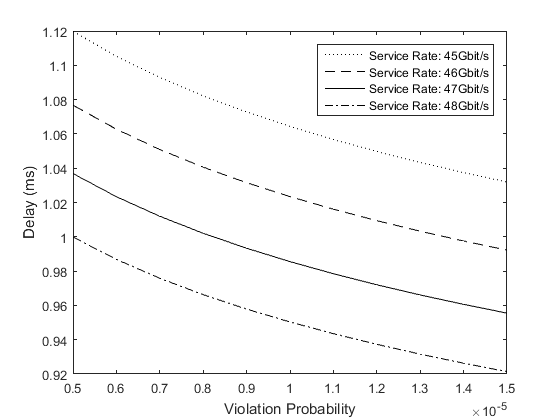
\includegraphics[width=.7\textwidth]{delay_no_tandem.png}
  \caption{Service Rate Influence}
  \label{fig2}
\end{figure}
Fig.\ref{fig2} provides the evaluated URLLC delay with different service rate under violation probability $1*10^{-5}$.
The value of violation probability is from $5*10^{-6}$ to $15*10^{-6}$.
We arrange the value scope to observe the effect of this value on delay.
We adopt 4 service rates in model and all the curves are slow down by violation probability value. From this, we can conduct that the violation probability is not the main factor to influence the latency.
In order to make the delay less than 1ms, we set service rate from 45Gbit/s to 48Gbit/s based on arrival rate 20Gbit/s.
We can procure that delay approximates 1ms when service rate is 47Gbit/s at violation probability $1*10^{-5}$.
As the service rate increases, the delay of the system will decrease.
When service rate is 48Gbit/s, system latency can approach 1ms with lower violation probability.
That means system can guarantee the low latency communication in a stable state.

\begin{figure}[htbp]
  \centering
  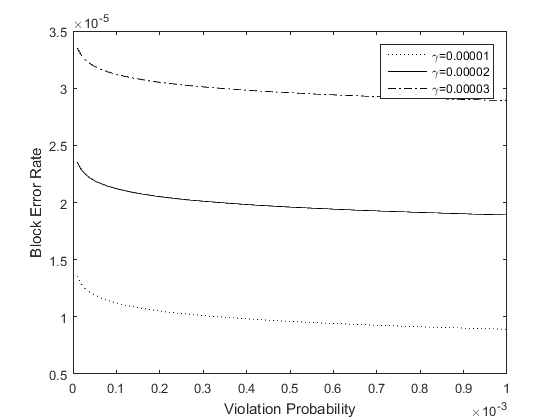
\includegraphics[width=0.7\textwidth]{BLER.png}
  \centering\caption{BLER Bound with parameter $\gamma$ }
  \label{fig_BLER}
\end{figure}
For Reliability of URLLC, we adopt SNC theory to study the stochastic bound of block error rate. In Fig.(\ref{fig_BLER}), we set the parameter $\gamma$ in three different values which is near to the $1*10^{-5}$. This parameter is set according to the BLER requirement of URLLC in 3GPP\cite{standard2}. We can get that the block error rate will decrease with the violate probability increasing. For the upper bound parameter $\gamma = 0.00001$, the BLER is well limited to the $1*10^{-5}$. It also means that the $99.999\%$ transmission correctness.

%add a new figure
\begin{figure}[htbp]
  \centering
  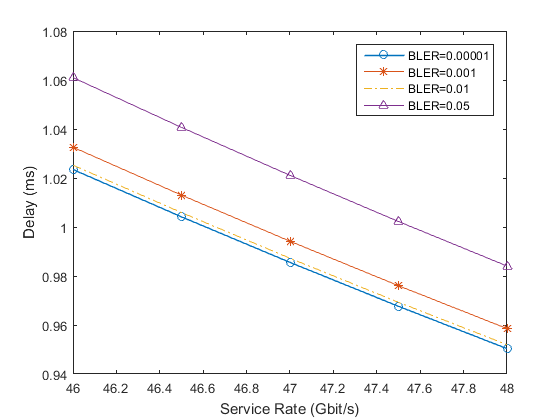
\includegraphics[width=.7\textwidth]{Delay_BLER.png}
  \centering\caption{Delay with Different BLER }
  \label{fig_Delay_BLER}
\end{figure}
Based on the reliability demand of URLLC, we study the influence of block error rate on system delay.
From Fig.\ref{fig_Delay_BLER}, we can see that BLER has little effect on the delay.
The delay varies very slightly when BLER value ranges from $1*10^{-5}$ to $1*10^{-3}$
A reason is that ultra reliability requires BLER not to exceed $1*10^{-5}$.
It is difficult for such a small value to have a large impact on service rate.
Thus the reliability of the system is guaranteed.

\begin{figure}[htbp]
  \centering
  \includegraphics[width=.7\textwidth]{Delay_Arrival.png}
  \centering\caption{Delay with Arrival Rate }
  \label{fig_Delay_Arrival}
\end{figure}

Fig.\ref{fig_Delay_Arrival} illustrates the relationship between system delay and service rate and arrival rate.
As shown in the figure, system delay raises with the increase of arrival rate.
When the arrival rate is 20Gbit/s, the system delay exceeds 1ms which is the requirement of URLLC.
With the increase of service rate, the system delay can be reduced to less than 1ms.
But when the arrival rate continues to increase, the delay will eventually exceed the demand.
Due to limited resources, service rates cannot increase infinitely.
Therefore, we should improve task scheduling and resource allocation.

\begin{figure}[htbp]
  \centering
  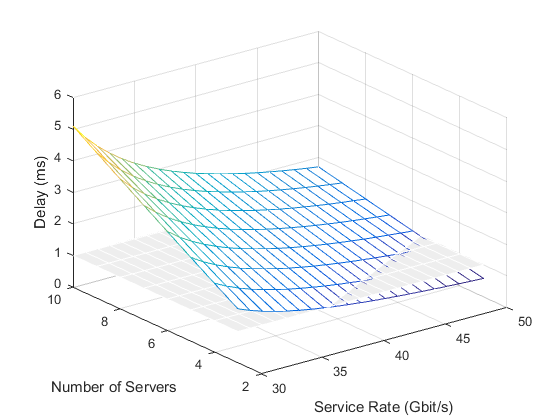
\includegraphics[width=.7\textwidth]{delay_servers.png}
  \caption{The Influence of Number of Tandem Servers on Delay}
  \label{fig3}
\end{figure}
Fig.\ref{fig3} presents the relationship among latency, number of server levels and service rate.
The arrival rate is constant and the speed is 20Gbit/s. The violation probability is maintained at $1*10^{-5}$.
Based on the above setting, we can derived that the delay is sensitive on number of tandem servers.
From Fig.\ref{fig3}, we can see the slope of latency caused by number of tandem servers is larger than the service rate.
We draw a delay equals 1ms flat plane to cut the curved surface.
The part below the plane is the scope of deployment parameters which satisfy the delay condition.
%This means that the delay is maintained below 1ms when the number of servers less than 5 at the same time service rate more than 40 Gbit/s.
This means that when the number of servers is less than 5 and the service rate is over 40 Gbit/s, the delay is maintained below 1 ms.
In order to ensure low latency of communication, it is necessary to reduce the number of tandem servers in deployment.
The edge computing is a popular deployment in 5G network. It is a typical example for reducing the number of servers in the transmission path.
Increasing server service rate is another way to reduce latency.
When the transmission rate is 20 Gbit/s, the service rate should be set above 40 Gbit/s.
In this way, the delay requirement of URLLC can be guaranteed.

The simulation experiment of the whole paper is mainly aimed at the performance requirements of URLLC.
In terms of Low-Latency, URLLC requires transmission delay less than or equal to 1 ms.
At the same time, in terms of Ultra-reliability, URLLC should ensure that the block error rate is $1*10^{-5}$.
Our simulation experiment reveals how to meet the requirements of latency and reliability.
In order to increase the transmission rate of the network to 20GBit/s, we need to meet the conditions in network construction.
The conditions like what kind of processing speed should the service rate of network nodes satisfy, and what range should be the number of hops
(tandem servers) from the access network to the cloud.

\section{Conclusions}
In this paper, the architecture of the 5G URLLC network is researched.
According to the architecture characteristics, the URLLC network is modeled as a tandem system which describes the communication from UE to Cloud.
Applying stochastic network theory and combining the features of URLLC network, performance analysis has been conducted.
We have investigated the relationship between delay constraint, service rate, violation probability, block error rate, and the number of deployed servers in URLLC network.
The 3GPP standard is taken into account when we set the simulation parameters.
Numerical results verify that the main factor which can impact latency is the number of servers deployed in tandem.
That also means Edge Computing will be the trend in URLLC application deployment.
The service rate of the server is also a factor affecting the delay.
With the increase of service rate, the delay can be reduced.
The results derived from evaluation provide valuable guidelines for the early design of URLLC deployment.
For our future work, we would consider to include handover access in URLLC communication.

% BibTeX users please use one of
%\bibliographystyle{spbasic}      % basic style, author-year citations
%\bibliographystyle{spmpsci}      % mathematics and physical sciences
%\bibliographystyle{spphys}       % APS-like style for physics
%\bibliography{}   % name your BibTeX data base


% Non-BibTeX users please use
\begin{thebibliography}{}
%
% and use \bibitem to create references. Consult the Instructions
% for authors for reference list style.
%
\bibitem{standard1} %1
ITU-R M.2083-0, IMT Vision - Framework and Overall Objectives of the Future Development of IMT for 2020 and Beyond (2015)
\bibitem{standard2} %2
 3GPP TR 38.913, Study on Scenarios and Requirements for Next Generation Access Technologies (2017)
\bibitem{article1} %3
Soldani D, Guo Y J, Barani B, et al., 5G for Ultra-Reliable Low-Latency Communications, IEEE Network, \textbf{32}(2), pp.6--7 (2018)
\bibitem{book1} %4
Jiang Y, Liu Y, Stochastic Network Calculus, Springer, London (2009)
\bibitem{article2} %5
M. Fidler and A. Rizk, A Guide to the Stochastic Network Calculus, IEEE Communications Surveys \& Tutorials, \textbf{17}(1), pp.92--105 (92-105)
\bibitem{article_interface}  %6
J. J. Nielsen, R. Liu and P. Popovski, Ultra-Reliable Low Latency Communication Using Interface Diversity, IEEE Transactions on Communications \textbf{66}(3), pp.1322-1334 (2018)
\bibitem{article_multiconnectivity}  %7
Delgado R A, Lau K, Middleton R H, et al., Networked Delay Control for 5G Wireless Machine-Type Communications Using Multiconnectivity, IEEE Transactions on Control Systems Technology \textbf{99}, pp.1--16 (2018)
\bibitem{article_PD}  %8
Rao J, Vrzic S, Packet Duplication for URLLC in 5G: Architectural Enhancements and Performance Analysis, IEEE Network \textbf{32}(2), pp.32--40 (2018)
\bibitem{article_Anand}  %9
Anand A, De Veciana G, Resource Allocation and HARQ Optimization for URLLC Traffic in 5G Wireless Networks, (2018)
\bibitem{article_Energy}    %10
Mukherjee A, Energy Efficiency and Delay in 5G Ultra-Reliable Low-Latency Communications System Architectures, IEEE Network \textbf{32}(2), pp.55--61 (2018)
\bibitem{article_joachim}   %11
Sachs J, Wikstrom G, Dudda T, et al., 5G Radio Network Design for Ultra-Reliable Low-Latency Communication, IEEE Network, \textbf{32}(2), pp.24--31 (2018)
\bibitem{proc_Huawei}  %12
Wang C, Chen Y, Wu Y, et al., Performance Evaluation of Grant-Free Transmission for Uplink URLLC Services, IEEE Vehicular Technology Conference 2017 Vtc2017-Spring,  pp.1--6 (2017)
\bibitem{article_Achieving}  %13
Pocovi G, Shariatmadari H, Berardinelli G, et al., Achieving Ultra-Reliable Low-Latency Communications: Challenges and Envisioned System Enhancements, IEEE Network, \textbf{32}(2), pp.8--15 (2018)
\bibitem{article_Wireless}  %14
Popovski P, Nielsen J J, Stefanovic C, et al., Wireless Access for Ultra-Reliable Low-Latency Communication: Principles and Building Blocks, IEEE Network, \textbf{32}(2), pp.16--23 (2018)
\bibitem{article_Introduction}  %15
Ji H, Park S, Yeo J, et al., Introduction to Ultra Reliable and Low Latency Communications in 5G, (2017)
\bibitem{article_Physical}  %16
Ji H, Park S, Yeo J, et al., Ultra Reliable and Low Latency Communications in 5G Downlink: Physical Layer Aspects, (2018)
\bibitem{article_jiang_power}  %17
Z. Li, Y. Jiang, Y. Gao, P. Li, L. Sang and D. Yang, Delay and Delay-Constrained Throughput Performance of a Wireless-Powered Communication System, IEEE Access, \textbf{5}, pp.21620--21631 (2017)
\bibitem{proc_MF_Estimation}  %18
R. L��bben and M. Fidler, Estimation method for the delay performance of closed-loop flow control with application to TCP, IEEE INFOCOM 2016-The 35th Annual IEEE International Conference on Computer Communications, pp.1--9 (2016)
\bibitem{article_beiyou_lei1}  %19
K. Zheng, F. Liu, L. Lei, C. Lin and Y. Jiang, Stochastic Performance Analysis of a Wireless Finite-State Markov Channel, IEEE Transactions on Wireless Communications \textbf{12}(2), pp.782--793 (2013)
\bibitem{article_si_yuan}   %20
Chen, Xin, Y. Si, and X. Xiang, Delay-bounded resource allocation for femtocells exploiting the statistical multiplexing gain, \textbf{71}, pp.3217--3236 (2015).
\bibitem{article_MF_jiang}  %21
M. Fidler, B. Walker and Y. Jiang, Non-Asymptotic Delay Bounds for Multi-Server Systems with Synchronization Constraints, IEEE Transactions on Parallel and Distributed Systems, \textbf{29}(7), pp.1545--1559 (2018)
\bibitem{article_Millimeter}  %22
Yang. Guang, M. Xiao, and H. V. Poor, Low-Latency Millimeter-Wave Communications: Traffic Dispersion or Network Densification?, IEEE Transactions on Communications, \textbf{66}(8), pp.3526--3539 (2018)
\bibitem{article_MF_Random}  %23
R. L��bben, M. Fidler and J. Liebeherr, Stochastic Bandwidth Estimation in Networks With Random Service, IEEE/ACM Transactions on Networking, \textbf{22}(2), pp.484--497 (2014)
\bibitem{article_WLE}  %24
Guly��s, Andr��s, B��r��, J��zsef, A stochastic extension of network calculus for workload loss examinations, Communications Letters IEEE, \textbf{10}(5), pp.399--401 (2006)
\bibitem{proc_Loss} %25
Deng Y, Lin C, An Extended Stochastic Loss Bound with Moment Generating Function, International Conference on Communications \& Mobile Computing IEEE (2010)
\bibitem{proc_infocom}  %26
Sami Ayyorgun, et al., A Composable Service Model With Loss and a Scheduling Algorithm, Infocom (2004)
\bibitem{proc_jiang_On}  %27
Wu K, Jiang Y, Li J, On the model transform in stochastic network calculus, In: International Workshop on Quality of Service IEEE, pp.1--9 (2010)
\bibitem{proc_jiang_Wireless}  %28
Sun F, Li L, Jiang Y, Impact of duty cycle on end-to-end performance in a Wireless Sensor Network, Wireless Communications and NETWORKING Conference IEEE, pp.1906--1911 (2015)
\bibitem{proc_Michael}  %29
Beck M, Towards the analysis of transient phases with stochastic network calculus, Telecommunications Network Strategy and Planning Symposium IEEE, pp. 164--169 (2016)
%\bibitem{RefJ}
% Format for Journal Reference
%Author, Article title, Journal, Volume, page numbers (year)
% Format for books
%\bibitem{RefB}
%Author, Book title, page numbers. Publisher, place (year)
% etc
\end{thebibliography}

\end{document}
% end of file template.tex

%
% For two-column wide figures use
%\begin{figure*}
% Use the relevant command to insert your figure file.
% For example, with the graphicx package use
  %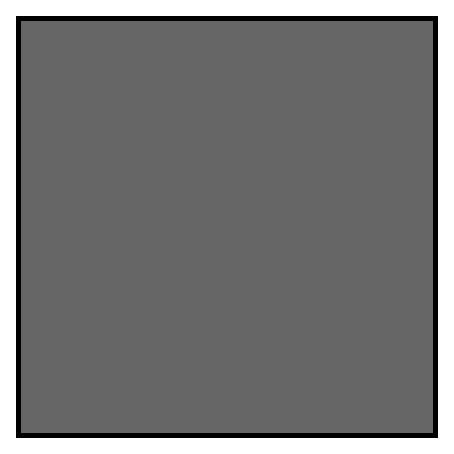
\includegraphics[width=0.75\textwidth]{example.eps}
% figure caption is below the figure
%\caption{Please write your figure caption here}
%\label{fig:2}       % Give a unique label
%\end{figure*}
%


% For one-column wide figures use
%\begin{figure}
% Use the relevant command to insert your figure file.
% For example, with the graphicx package use
  %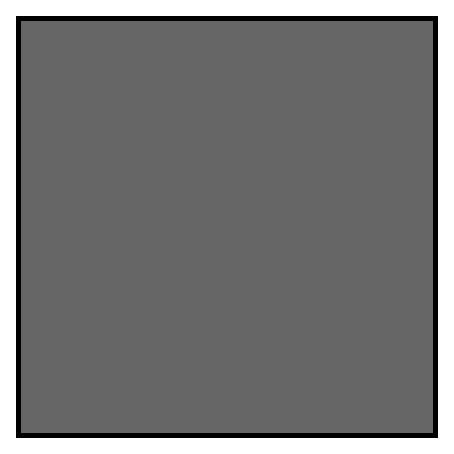
\includegraphics{example.eps}
% figure caption is below the figure
%\caption{Please write your figure caption here}
%\label{fig:1}       % Give a unique label
%\end{figure}

